%!TEX root = ../../../adrien_gomar_phd.tex

\chapter{Conditioning of multi-frequential harmonic balance methods}
\label{cha:limitations_condition_number}

\chabstract{
Problems characterized by multiple frequencies require 
multi-frequential harmonic balance discretization operators.
These can be ill-conditioned for some combinations 
of the discrete frequencies.
In this chapter, we investigate the sensitivity of 
harmonic balance solutions to the condition number of the 
discrete Fourier transform matrix for a linear advection problem
and a non-linear channel flow problem.
Highlighted is the fact that when the condition number is greater
than one, the unsteadiness can be badly reproduced preventing the use
of such an approach.
To improve the condition number, we consider a non-uniform
distribution of the times instances (\citet{ThesisGuedeney}),
along with an optimization algorithm minimizing the
condition number of the discrete Fourier transform matrix.
The optimization algorithm developed
in the present work gives very good results for any input frequencies,
enabling the use of the multi-frequential harmonic balance
for the simulation of contra-rotating open rotor aeroelasticity.
This work has been published:
\newline

\noindent
T. Gu\'edeney, \emph{A. Gomar}, F. Gallard, F. Sicot, G. Dufour, and G. Puigt. 
Non-Uniform Time Sampling for Multiple-Frequency Harmonic Balance Computations. 
\emph{Journal of Computational Physics}, 236:317--345, March 2013} 


\newpage

\section{Condition number and contra-rotating open rotor aeroelasticity}
\label{sec:condition_cror_ael}
%!TEX root = ../../../adrien_gomar_phd.tex

As shown previously in Sec.~\ref{sec:cror_unsteady}, the main unsteady
phenomena encountered in CROR can be correlated with the blade passing
frequency.
In addition to that, the aeroelastic phenomenon
studied here, namely blade flutter sensibility, has a vibration frequency that
is imposed (forced movement simulation) that depends on the proper modes
of the structure (see Sec.~\ref{sub:flutter}).
In general, these are not harmonically related nor
of the same order of magnitude. Hence the use of the
multi-frequential formulation of the HB approach. 

The condition number $\kappa$ of a matrix $A$ is defined as:
\begin{equation}
  \kappa (A) = \kappa (A^{-1}) = \| A \| \cdot \| A^{-1} \|, \quad
    \kappa(A) \geq 1,
\end{equation}
where $\| \cdot \|$ denotes a matrix norm. Considering the resolution
of the system of equation
$A x = b$, if $A$ is invertible and if $\delta A$, $\delta x$ and
$\delta b$ are the numerical errors associated with the computation of
$A$, $x$ and $b$, respectively, then:
\begin{equation}
   (A + \delta A)(x + \delta x) = b + \delta b.
   \label{eq:error_reso}
\end{equation}
By definition, the condition number sets an upper bound for 
the error made on~$x$:
\begin{equation}
   \frac{\| \delta x \|}{\| x \|} \leq 
   \kappa(A)\left[\frac{\| \delta A \|}{\| A \|} + 
   \frac{\| \delta b \|}{\| b \|} \right].
   \label{eq:conditonnig_amp}
\end{equation}
By transposing this to our problem, namely $A$ is the residual, 
$b$ the source terms and $x$ the conservative variables, one can say that
the error on the iterative resolution of the governing equations can
therefore be amplified by the harmonic balance source term.
Using the definition given in Eq.~\eqref{eq:conditonnig_amp}, this amplification is
led by the condition number of the DFT matrix $E$. 


In the mono-frequential formulation, the logical sampling is the uniform one
which has the good property of providing
a well conditioned DFT matrix $E$. In fact, in this framework, $E$ is orthogonal giving 
the smallest condition number $\kappa (E) = 1$
In the multi-frequential framework,
the condition number of the DFT matrix $E$ is not always unity and
varies under frequencies and time instances change~\cite{Kundert1988}. 
The frequencies
being imposed by the problem that is simulated,
the only degrees of freedom left to control the condition
number are the time instances. 
Moreover, the amplitude of the unsteadinesses, represented by $\delta x$
can not be \emph{a priori} controlled as this is ruled by the flow physics. 
Therefore, the condition
number must be minimized using the time instances.

All variations of the HB approach proposed in the literature rely on 
a uniform time sampling of the longest period of interest 
(though the number of samples can differ). 
This uniform time sampling can raise stability issues.
To emphasis this, let us consider two independent frequencies $f_1$
and $f_2$ that plays the role, respectively, of the blade passing frequency and
the vibration frequency. The two frequencies are arbitrarily chosen between~1
and $10,000$~Hz and the corresponding
condition number of the DFT matrix $E$ is compute. The results using a uniform time
sampling is shown in Fig.~\ref{fig:algo_equi_assessment}.
100~points are used to discretize each frequency interval giving a frequency step
of 100~Hz.
The problem being symmetric in $(f_1, f_2)$, so are the results.
Moreover, the structure of the results seems to indicate that only the
ratio of $f_2$ over $f_1$ is important as the shape of the
solution is constant under a translation of vector $(1,1)$.

Almost half of the set of frequencies have a DFT matrix $E$
whose condition number is superior to ten.
The minimum values are obtained with harmonically related couple
of frequencies. In fact, the white zones in Fig.~\ref{fig:algo_equi_assessment}
are the regions where $f_2 = n f_1$ with $n \in \mathbb{N}$ or $1/n \in \mathbb{N}$.
Elsewhere, the condition number is large and grows exponentially.
\begin{figure}[htp]
  \centering
  \includegraphics*[width=0.5\textwidth]{algo_equi_assessment.pdf}
  \caption{Condition number of the discrete Fourier transform matrix $E$
  using two independent frequencies and evenly space time instances.}
  \label{fig:algo_equi_assessment}
\end{figure}
To highlight this, the minimum, maximum, mean and 
standard deviation (noted $\sigma$) values of the
previous example are summarized in Tab.~\ref{tab:hb_algo_equi}.
\begin{table}[htp]
  \ra{1.3} 
  \centering
  \begin{tabular}{cccc}
    \toprule
    min & max & mean & $\sigma$ \\
    \midrule
    $1.0$ & $9.4\e{16}$ & $1.5\e{14}$ & $2.8\e{15}$ \\
    \bottomrule
  \end{tabular}
  \caption{Condition number of the discrete Fourier transform matrix $E$: 
  statistics for two independent frequencies using evenly spaced time instances.}
  \label{tab:hb_algo_equi}
\end{table}  
The values of the maximum, mean and standard deviation are tremendous
and the standard deviation is greater than the mean
($\sigma > $ mean) preventing the blindly use of such a sampling strategy for 
multi-frequential HB computations.
In numerical methods, it is common to deal with ill-conditioned
problems. However, we will show below that HB results are 
very sensitive to the condition number of the DFT matrix $E$.
To do so, the linear advection toy problem
presented in Chap.~\ref{cha:toy_problems},
is used with varying condition number and input unsteadinesses.


\section{Highlighting the problem}
\label{sec:condition_pbm}
%!TEX root = ../../../adrien_gomar_phd.tex
\paragraph{Using the advection equation model problem}

A pure harmonic signal is imposed at the left boundary condition
of the linear advection equation toy problem presented in Sec.~\ref{sec:toy_convection}:
\begin{equation}
   u_l (t) = 1 + \sin \left(2 \pi f t\right).
\end{equation}
The minimal condition number
$\kappa(E) = 1$ is obtained with evenly spaced time instances.
In fact, as the injected function is mono-frequential, 
the theoretical lower bound of the condition number is obtained by using evenly
spaced time instances.
The time instances of the harmonic balance
computations are chosen to reach varying condition numbers
such that $1 \leq \kappa (E) \leq 10$.  

As shown in the previous section, the condition number 
can, by definition, amplify the error made
on the iterative resolution of the linear advection equation.
This is illustrated in Fig.~\ref{fig:condition_number_local_amp} which 
shows the evolution of the results with a varying condition number.
The amplitude of the
sinusoidal function is either under or over-estimated when
$\kappa (E) \neq 1$. However, 
the higher the condition number, the worse the accuracy in capturing
the amplitude of the injected function. Moreover, when $\kappa(E) \geq 6$,
the shape of the solution is even inverted which would lead to
bad conclusions if analyzed as it.
\begin{figure}
  \centering
  \includegraphics*[width=0.50\textwidth]{condition_number_local_amp.pdf}
  \caption{Linear advection of a sinusoidal function: numerical steady-state 
  solutions at $t=0$ for varying condition number.}
  \label{fig:condition_number_local_amp}
\end{figure}

\paragraph{Using the channel flow toy problem}
The previous example was based on the advection equation which
has the good property of having a analytical solution to 
analyze the results. The results show that the harmonic
balance solutions are very sensitive to the condition number.
To further analyze the condition number issue,
the unsteady channel flow toy problem
(see Sec.~\ref{sec:toy_channel}) is computed with a single
frequency oscillating back-pressure 
at the outlet: $f_1 = 3$~Hz, the second
frequency having a zero amplitude: $a_2= 0$:
\begin{equation}
   P_{outlet} (t) = P_m \left[ 1 + a_1 \sin \left(2 \pi f_1 t\right) \right].
\end{equation}
This helps understanding the behavior of the HB source term
within the Navier--Stokes equations framework.

As the oscillating back-pressure is composed of only one frequency,
it is mono-frequential.
Thus, by using evenly-space time instances, the condition
number of the source term is unity $\kappa (E) = 1$. 
To highlight the issue related to the condition number,
the time instances are chosen to reach varying condition numbers
such that $1 \leq \kappa (E) \leq 3.43$.  
Two frequencies are
specified for the HB computation: $f_1$ and its first harmonic
$2f_1$. 


\begin{figure}
  \centering
  \subfigure[$a_1 = 0.01$]{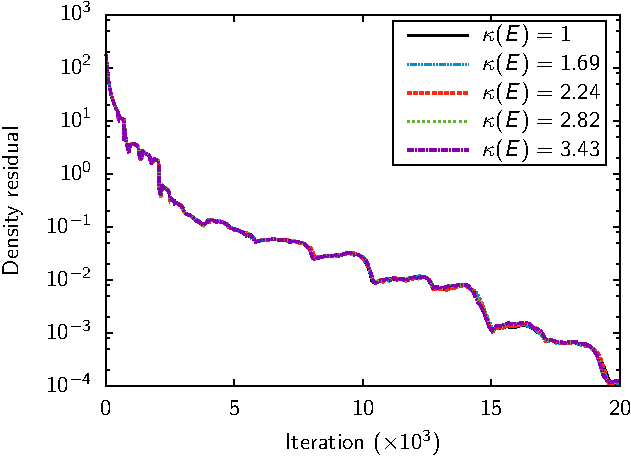
\includegraphics[width=.45\textwidth]{CANAL2_RESIDUAL_VS_CONDITIONNING_AMP001_PPT.pdf}}
  \subfigure[$a_1 = 0.05$]{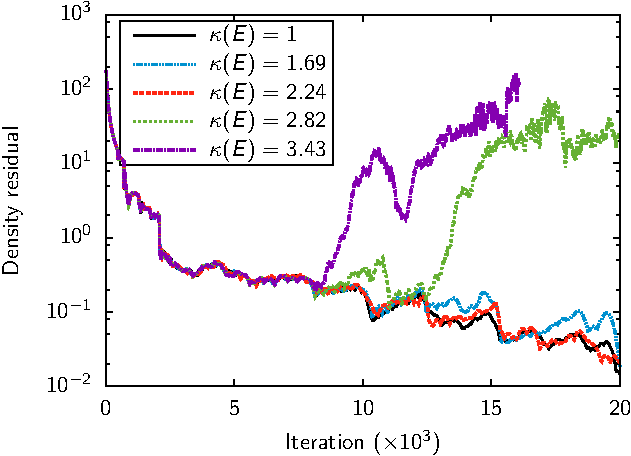
\includegraphics[width=.45\textwidth]{CANAL2_RESIDUAL_VS_CONDITIONNING_AMP005_PPT.pdf}}
  \caption{Relation between the condition number $\kappa (E)$ and the convergence of the solution.}
  \label{fig:canal_residual_vs_conditionning}
\end{figure}
The results in Fig.~\ref{fig:canal_residual_vs_conditionning} show that
for a condition number $\kappa (E) \geq 2.24$ and wave input amplitude
$a_1 = 0.05$, the computation diverges. However, the computations with
the same condition numbers but a smaller input amplitude $a_1 = 0.01$
converge. In fact, the condition number amplifies the errors made
during the iterative process. When the input waves have a smaller
amplitude, the iterative errors are slighter.

The problem is that for a given configuration, the amplitude of the computed unsteady phenomena can not
be \emph{a priori} known. This is emphasized in the section bellow
as in the literature, the condition number of the computations
has been almost $20$ and still the simulations converge.

\paragraph{Literature review}
\label{sec:condition_literature}

In the turbomachinery literature, \citet{Gopinath2007} and
\citet{Ekici2007} assessed their implementation of the
HB method on a 2D multi-stage compressor. 
It is composed of a rotor sandwiched by two stators having
32, 40 and 50~blades, respectively. Various combinations of the stators
blade passing frequencies are considered, 
but always with evenly-spaced time instances sampling the
largest period.  While \citet{Gopinath2007} use $2N+1$ samples (noted EVE $2N+1$),
\citet{Ekici2007} over-sample this period with $3N+1$ time instances
(noted EVE $3N+1$). This
leads to a rectangular $(2N+1)\times(3N+1)$ almost-periodic Fourier
matrix that gives thus HB computations that are more CPU and memory demanding
(see Sec.~\ref{sec:sm_hb_cost}). 
The chosen frequencies and the \emph{a posteriori}
associated condition numbers of the above references are given in
Tab.~\ref{tab:literature_multistage}.  
In bold text is highlighted the condition number used in the
original computations.
For $N=4$, the $3N+1$ instants
oversampling approach of \citet{Ekici2007} efficiently reduces the
condition number. But for this case, the use of evenly-spaced time
instances is sufficient as the condition number seems to be small enough
for the considered magnitude of unsteadiness.
\begin{table}
  \centering
  \begin{tabular}{rcc}
    \toprule
    \multicolumn{1}{c}{Reference} & \multicolumn{2}{c}{$\kappa(E)$} \\
    \multicolumn{1}{c}{and \# harmonics} & EVE $(2N+1)$ & EVE $(3N+1)$ \\
    \midrule
    \citet{Gopinath2007} ($N=2$) & $\mathbf{3.79}$ & $3.00$ \\
    \citet{Ekici2007} ($N=3$) & $5.40$ & $\mathbf{3.84}$ \\
    \citet{Gopinath2007} ($N=4$) & $\mathbf{11.25}$ & $2.07$ \\
    \citet{Gopinath2007} ($N=7$) & $\mathbf{16.66}$ & $14.61$ \\
    \bottomrule
  \end{tabular}
  \caption{Literature review of the condition number used in multi-frequential
  harmonic balance computations.}
  \label{tab:literature_multistage}
\end{table}

However, such an approach fails when dealing with configurations where:
\begin{itemize} \itemsep0pt \parskip0pt
  \item the amplitude of unsteadinesses is large as for instance
  large oscillations of a blade,
  \item the frequencies are widely segregated. In fact, as shown previously
  in Sec.~\ref{sec:condition_cror_ael}, the more segregated the frequencies, the
  higher the condition number using a uniform time sampling. This condition number
  can be tremendous ($\kappa (E) \ll 100$) preventing the use of such
  an approach for given configurations.
\end{itemize}

Moreover, as the amplitude of unsteadinesses plays a crucial role in
the amplification done by the condition number, the only
way to ensure that a simulation will converge is 
to minimize the condition number.
Therefore, the section below will be dedicated to
the development of algorithms to achieve this goal.


\section{Proposed cure: automatic optimization of time instances} % (fold)
\label{sec:condition_solution}
%!TEX root = ../../../adrien_gomar_phd.tex

Two algorithms that automatically choose the time instances in order to
minimize the condition number are presented: first, the Almost
Periodic Fourier Transform (APFT) algorithm, initially proposed in the
literature for electronics problems and implemented by
\citet{ThesisGuedeney} in his PhD thesis, is described, then a gradient-based
optimization algorithm over the condition number (OPT), developed in
the current work, is presented.

\subsection{Almost-Periodic Fourier Transform algorithm (APFT)}
\label{sec:apft_algorithm}
Based on the work of \citet{Kundert1988} in
electronics, the APFT
algorithm has been implemented by \citet{ThesisGuedeney} 
during his PhD thesis. The algorithm is designed
to maximize the orthogonality of the multi-frequential
IDFT matrix in order to minimize its condition number. To do so, a
Gram-Schmidt orthogonalization procedure is conducted.  First, the period 
associated with the smallest frequency ($2 \pi / \omega_{min}$) 
is oversampled with $M$ evenly spaced time
instances, $M\gg2N+1$ being specified by the user with $N$ the number of
frequencies. Considering these time instances, a rectangular
multi-frequential IDFT matrix is built. This rectangular matrix can be seen
as a set of $M$ vectors of length $2N+1$.
The first vector noted $V_0$ (corresponding
to $t=0$) is arbitrarily chosen as the first time instance and any
component in the direction of $V_0$ is removed from the following
vectors using the Gram-Schmidt formula
\begin{equation}
   V_s = V_s - \frac{V_0^\top V_s}{V_0^\top V_0} V_0, \quad s=1 \cdots M-1.
   \label{GramSchmidtAlgo}
\end{equation}
The remaining vectors are now orthogonal to $V_0$. 
Initially, the vectors had the same Euclidean norm.
Therefore, the vector that has now the largest norm is
the most orthogonal to $V_0$.
It is thus assigned to $V_1$. The previous
operations are then performed on the $M-2$ remaining vectors using $V_1$
as starting point. This process is repeated until the required $2N+1$ vectors
are defined. As a time instance corresponds to a vector, $2N+1$ time instances are obtained, 
which enables the construction of the multi-frequential
IDFT matrix. This algorithm is summarized in
Algo.~\ref{alg:algo_APFT}.

\begin{algorithm}
\caption{The Almost Periodic Fourier Transform Algorithm (APFT)}
\label{alg:algo_APFT}
\begin{algorithmic}
\STATE $\omega_{min} \leftarrow min \left( |\omega_k |,\quad 1 \leqslant k \leqslant N \right)$
\FOR{$m \leftarrow 0 \cdots M-1$}
    \STATE $t_m \leftarrow \displaystyle\frac{2\pi}{\omega_{min}}\frac{m}{M}$
\ENDFOR
\FOR{$n \leftarrow 1 \cdots 2N$}
   \FOR{$m \leftarrow n+1 \cdots M$}
  \STATE $ V_{m} \leftarrow V_{m} - \displaystyle\frac{V_{n}^\top \cdot V_{m}}{V_{n}^\top \cdot V_{n}} V_{n}$
   \ENDFOR
   \STATE \textbf{argmax()} returns the index of the largest member of a set
   \STATE $k=\textbf{argmax} \left( \| V_s^n \|,\quad n+1\leqslant s \leqslant M\right) $
   \STATE $\textbf{swap}(V_{n+1},V_{k})$
   \STATE $\textbf{swap}(t_{n+1},t_{k})$
\ENDFOR
\STATE $\mathbb{T}_{optimized} \leftarrow [t_0 \cdots t_{2N}]$
\end{algorithmic}
\end{algorithm}

\subsection{Gradient-based optimization algorithm (OPT)}
\label{sec:algo_opt}
A more direct approach is to seek directly a set of time instances
that minimize the condition number of the associated multi-frequential IDFT matrix. 
This minimization problem can be solved numerically by an optimization algorithm.

The limited memory optimization method of
\citet{Byrd1995} (noted L-BFGS-B) is
used to look for a minimum of the condition number of the
multi-frequential IDFT matrix $\kappa \left(E^{-1} \left[\mathbb{T} \right]
\right)$ as function of the time instances vector $\mathbb{T}$. This
quasi-Newton algorithm approximates the inverse Hessian matrix
$H(\kappa \left(E^{-1} \left[\mathbb{T} \right] \right))^{-1}$ with the
BFGS formula in order to decrease the objective $\kappa \left(E^{-1}
  \left[\mathbb{T} \right] \right)$ in the direction $-H(\kappa
\left(E^{-1} \left[\mathbb{T} \right] \right))^{-1}\nabla \kappa \left(E^{-1}
  \left[\mathbb{T} \right] \right)$. In the present case, the
derivative $\nabla \kappa \left(E^{-1} \left[\mathbb{T} \right] \right)$ of
the objective with respect to the time instances is approximated by
a first-order finite differences. The descent direction is
associated with the search for a zero of the gradient, which is a
necessary condition for an extrema, in a second-order Taylor series.
Finally, a line search on $\alpha$ is performed to minimize $\kappa
\left(E^{-1} \left[\mathbb{T} - \alpha H(\kappa \left(E^{-1} \left[\mathbb{T}
      \right] \right))^{-1} \nabla \kappa \left(E^{-1} \left[\mathbb{T}
      \right] \right) \right] \right)$.  An open-source implementation of this
broadly-used algorithm is
employed~\cite{Nocedal1980}.

Gradient descent methods being local, the L-BFGS-B method converges to a local
minimum of the condition number. This minimum is unsatisfying if the
starting time instances vector $\mathbb{T}$ is not well chosen, therefore a strategy
to find an appropriate initial point is required. To this aim, the smallest
angular frequency $\omega_{min}$ is used as a base angular frequency to create a set $\Omega$
\begin{equation}
    \Omega = [\frac{1}{M} \omega_{min} \cdots \frac{m+1}{M} \omega_{min} \cdots \omega_{min}],
    \label{eq:slitted_period}
\end{equation}
where $M$ denotes the desired number of initial guesses.
This gives a set of periods. Each of them are then evenly sampled to obtain a
set of time instances $\mathbb{T}_m$
\begin{equation}
    \mathbb{T}_m = \left[ 0, \frac{2 \pi M}{ (2N + 1) (m+1) \omega_{min}} \cdots 
                             \frac{2N \pi M}{ (2N + 1) (m+1) \omega_{min}} \right]
    \label{eq:set_of_tlv}
\end{equation}
These time instances sets are finally used as initial guesses for the
L-BFGS-B algorithm.

The multi-frequential IDFT matrix is then built for
each one of these time instances and the corresponding condition numbers are
computed. A large number $M$, typically thousands, of fractions of the
greatest period gives a large set of potential time instances vectors.
This is acceptable given the very low cost of the computation of the
condition number on such small matrices of size $(2N + 1) \times
(2N+1)$.  From this set, the time instances vector associated with the
multi-frequential IDFT matrix having the smallest condition number is
taken as a starting point.  The optimization algorithm actually achieves
a local adjustment of the time instances.

In this way, the exploitation capability of the gradient-based
optimizer is well combined with the exploration capacity of the
sampling. The OPT algorithm is summarized in Algo.~\ref{alg:algo_opt}.
\begin{algorithm}
\caption{The gradient-based optimization algorithm (OPT)}
\label{alg:algo_opt}
\begin{algorithmic}
\STATE $\omega_{min} \leftarrow min \left( |\omega_k |,\quad 1 \leqslant k \leqslant N \right)$
\FOR{$m \leftarrow 0 \cdots M - 1$}
    \STATE $\omega_m \leftarrow \frac{m + 1}{M} \cdot \omega_{min}$
    \FOR{$i \leftarrow 0 \cdots 2N$}
        \STATE $t_i \leftarrow \displaystyle\frac{i \cdot 2 \pi}{\omega_m \cdot (2N + 1)}$
    \ENDFOR
    \STATE $\mathbb{T}_m \leftarrow [t_0 \cdots  t_i \cdots t_{2N}]$
    \STATE $C_m \leftarrow \kappa \left(E^{-1} \left[\mathbb{T}_m \right] \right)$
\ENDFOR
\STATE \textbf{argmin()} returns the index of the smallest member of a set
\STATE $k \leftarrow \textbf{argmin}\left(C_m,\quad 0\leqslant m \leqslant M-1\right)$
\STATE $\textbf{min\_l-bfgs-b}\left(\kappa \left(E^{-1} \left[\mathbb{T}\right]\right), \mathbb{T}_{ini}\right)$ returns the optimal 
time instances vector $\mathbb{T}$ using the condition number $\kappa\left(E^{-1} \left[\mathbb{T}\right]\right)$ as objective function 
for the L-BFGS-B algorithm and  $\mathbb{T}_{ini}$ as starting point.
\STATE $\mathbb{T}_{optimized} \leftarrow 
  \textbf{min\_l-bfgs-b}\left(\kappa\left(E^{-1} \left[\mathbb{T}\right]\right), \mathbb{T}_{ini}=\mathbb{T}_k\right)$
\end{algorithmic}
\end{algorithm}

\subsection{Assessment of the algorithms}
Taking the same independent couple of frequencies $(f_1, f_2)$ as the one
used is Sec.~\ref{sec:condition_cror_ael}, the condition number of the
multi-frequential DFT matrix $\kappa (E)$ is computed, highlighting
the ability of the different algorithms to choose the time instances that
minimize the condition number, for any input frequencies. This
assessment is only made for two frequencies, but the results are similar
when increasing the number of frequencies. As two frequencies are
involved, five time instances are required. The results for the three
algorithms are depicted in Figure~\ref{fig:bench_algo}: (i)~APFT: the
Almost Periodic Fourier Transform algorithm, (ii)~OPT: the
gradient-based OPTimization algorithm and (iii)~EVE: EVEnly spaced
time instances oversampling the largest period as done in
\citet{Gopinath2007} using $2N+1$ time
instances and in \citet{Ekici2007} and \citet{Ekici2008} using $3N+1$
time instances.
Table~\ref{tab:algo_sum} gives some statistics about the results obtained
with each algorithm to give the reader a quantitative overview of the
efficiency of the different algorithms.
\begin{figure}[htp]
  \centering 
    \subfigure[EVE $(2N + 1)$]{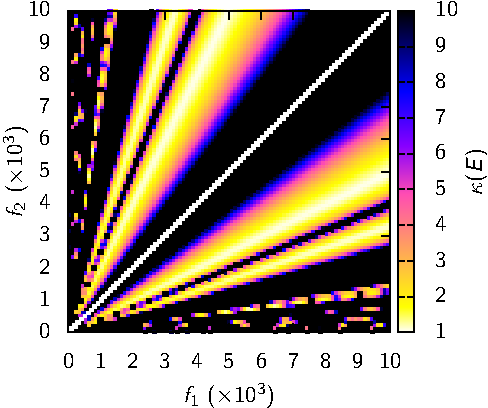
\includegraphics[width=.45\textwidth]{algo_equi_assessment.pdf}}
    \subfigure[EVE $(3N + 1)$]{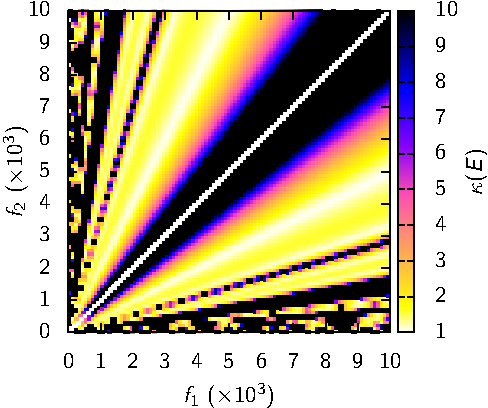
\includegraphics[width=.45\textwidth]{algo_equi_3n_assessment.pdf}}
    \subfigure[APFT]{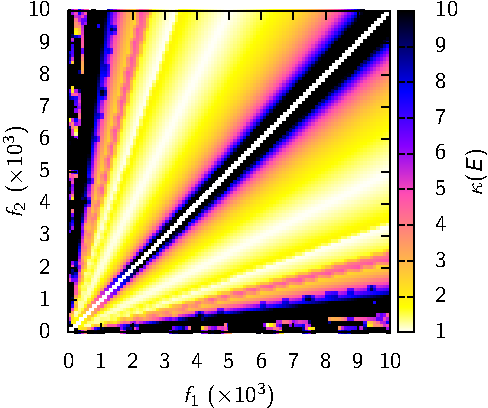
\includegraphics[width=.45\textwidth]{algo_apft_assessment.pdf}}
    \subfigure[OPT]{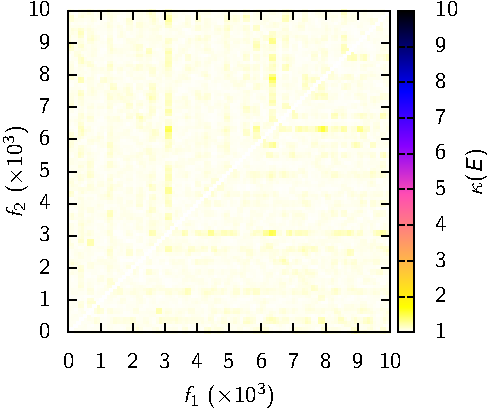
\includegraphics[width=.45\textwidth]{algo_opt_assessment.pdf}}
  \caption{Condition number of the discrete Fourier transform matrix $E$
  using two independent frequencies and four different algorithms
  to choose the time instances.}
  \label{fig:bench_algo}
\end{figure}

The EVE algorithms give fair results ($\kappa(E) \leq 2$) only at
discrete couples of frequencies, corresponding 
to the particular cases where $f_2$ is a
multiple of $f_1$, as shown in Sec.~\ref{sec:condition_cror_ael}. 
This is not promising as these
cases can be computed using the mono-frequential formulation and thus does not
need non-uniform time instances. Oversampling improves the results. 
In fact, the mean condition number obtained
with $3N + 1$ samples indicates that the higher the number of time instances
the better the condition number. However the multi-frequential DFT
matrix becomes rectangular. The memory and CPU cost being proportional to 
the number of time instances (see Sec.~\ref{sec:sm_hb_cost}), 
such a strategy can not be
used in an industrial context. The APFT
algorithm improves the results, as it gives $\kappa (E) \leq 2$ 
for a large interval but fails when the frequencies
are too close from one another ($f_1 \approx f_2$) or when they are significantly
different ($f_1 \ll f_2$ or $f_1 \gg f_2$).  
Finally, the OPT algorithm gives a condition number close to unity for
all couple of frequencies $(f_1, f_2)$. Moreover, the OPT algorithm is
the only one to give a standard deviation that is smaller than the mean,
proving its robustness.
\begin{table}[htp]
  \ra{1.3} 
  \centering
  \begin{tabular}{lcccc}
    \toprule
    \phantom{abdefghijk} & min & max & mean & $\sigma$ \\
    \midrule
    EVE ($2N + 1$) & $1.0$ & $9.4\e{16}$ & $1.5\e{14}$ & $2.8\e{15}$ \\
    EVE ($3N + 1$) & $1.0$ & $3.7\e{16}$ & $4.7\e{13}$ & $9.5\e{14}$ \\
    APFT & $1.0$ & $81.2$ & $5.9$ & $9.0$ \\
    OPT & $1.0$ & $2.6$ & $1.1$ & $7.7\e{-2}$ \\
    \bottomrule
  \end{tabular}
  \caption{Condition number of the discrete Fourier transform matrix $E$
  statistics for two independent frequencies using four different algorithms
  to choose the time instances.}
  \label{tab:algo_sum}
\end{table} 

The configurations encountered in the turbomachinery literature 
are taken again to demonstrate the capability of the presented
algorithms to minimize the condition number
regardless of the input frequencies. The results are shown in 
Tab.~\ref{tab:literature_multistage2}.
The APFT algorithm improves the condition number compared to the
EVE ($2N+1$) but can give relatively large condition numbers, here $12.95$. 
In opposite, the OPT algorithm developed in the
present contribution gives results close to one for the four configurations.
\begin{table}[htp]
  \ra{1.3} \centering
  \begin{tabular}{rcccc}
    \toprule
    \multicolumn{1}{c}{Reference} & \multicolumn{4}{c}{$\kappa(E)$} \\
    \multicolumn{1}{c}{and \# harmonics} & EVE $(2N+1)$ & EVE $(3N+1)$ & APFT & OPT \\
    \midrule
    \citet{Gopinath2007} ($N=2$) & $\mathbf{3.79}$ & $3.00$ & $1.72$ & $1.08$ \\
    \citet{Ekici2007} ($N=3$) & $5.40$ & $\mathbf{3.84}$ & $1.71$ & $1.00$ \\
    \citet{Gopinath2007} ($N=4$) & $\mathbf{11.25}$ & $2.07$ & $3.46$ & $1.13$ \\
    \citet{Gopinath2007} ($N=7$) & $\mathbf{16.66}$ & $14.61$ & $12.95$ & $1.00$ \\
    \bottomrule
  \end{tabular}
  \caption{Literature review of the condition number used in multi-frequential
  harmonic balance computations compared to the presented algorithms.}
  \label{tab:literature_multistage2}
\end{table}

% Thus the proposed non-uniform time sampling combined with the OPT
% algorithm allows to tackle problems with large frequency
% separation. In such cases, the gain of the HB approach compared
% to classical time-marching methods is expected to be significant: with
% a time-marching scheme, the time-step has to be small enough to
% discretize the shortest period, while the number of time steps of the
% simulation has to be long enough to reach the steady-state
% (\emph{i.e.}  the simulation time is equal to several
% times the longest period). Conversely, as detailed in Sec.~\ref{sec:sm_hb_cost},
% the cost of the HB method only
% depends on the number of frequencies to capture, regardless of their
% relative values.

Thus, the non-uniform time sampling proposed by \citet{ThesisGuedeney}
used together with the OPT algorithm developed in the present contribution
enables to tackle problems with large frequency separation and/or large unsteadinesses,
namely CROR aeroelasticity.

\subsection{Distribution of the time instances}
For harmonically-related frequencies, the set of time instances
that minimize the condition number is 
provided by a uniform sampling of the fundamental frequency period
as it gives the theoretical lower bound $\kappa (E) = 1$. Since the
frequencies are harmonically related, the distribution of the time
instances on the other frequencies is also uniform. 
In fact, considering the
frequency vector $F = \left[f_1 \cdots f_k= kf_1 \cdots Nf_1 \right]$
and the time instances vector
$\mathbb{T}$ uniformly sampling the smallest frequency
\begin{equation}
  \mathbb{T} = \left[0, \frac{1}{f_1 (2N+1)} \cdots  \frac{2N}{f_1 (2N+1)} \right],
  \label{eq:evenly_spaced_timelevels}
\end{equation}
then the product of the $i^{th}$ term of $\mathbb{T}$ to its
associated frequency is
\begin{equation}
  f_1 \frac{i}{f_1 (2N+1)} = k f_1 \frac{i}{k f_1 (2N+1)} = f_k \frac{i}{f_k (2N+1)}.
  \label{eq:evenly_spaced_timelevels_2}
\end{equation}
Equation~\eqref{eq:evenly_spaced_timelevels_2} means that evenly-spaced
time instances for the fundamental frequency are still seen as evenly
spaced by the $k^{th}$ harmonic. This is an explanation why the
condition number of the multi-frequential IDFT matrix $E^{-1}$ will be
unity as each frequency is sampled by evenly spaced time
instances~\cite{Brambilla1999}.

Now, considering non-harmonically related frequencies, there is
mathematically no reason for evenly-spaced time instances over the
smallest frequency to be seen as evenly spaced by the other frequencies
in general.

Figure~\ref{fig:distribution_tlv} shows the distribution of the time
instances, relative to each frequency period, obtained by the presented
algorithms for the frequencies $f_1 = 3$~Hz and $f_2 = 17$~Hz. 
To do so, the chosen time instances are redistributed
on the considered frequency period by applying a modulo to it
\begin{equation}
  \label{eq:1}
  \mathbb{T}^{[f_k]}_j =  \mathbb{T}_j \text{ modulo } 1/f_k
\end{equation}
Then, they are divided by the latter, so that the results are
dimensionless.  In light gray line is depicted the $y=x$ function
representing the evenly-spaced solution on the considered period.
Keeping in mind that if each frequency sees evenly-spaced time instances,
then the condition number is the smallest, the optimal solution would
be to have relative time instances on $y=x$ for each period.  Running the
EVE $(2N + 1)$, APFT and OPT algorithms leads to a condition number of $33.1$,
$3.8$ and $1.1$, respectively.  The EVE algorithm gives a perfect distribution
of the time instances with respect to
period $1/f_1$ as the time instances are sampled on the period
$1/f_1$. However, it gives results that are far from the evenly spaced time instances
within period $1/f_2$. The APFT algorithm is nowhere near the evenly spaced
solution for both the considered periods, but closer than EVE regarding
period $1/f_2$. Finally, the OPT algorithm is the only one to be close
to the evenly spaced solution for each period considered. This explains the
very good condition numbers obtained with the OPT algorithm.
\begin{figure}[htp]
  \centering 
  \subfigure[relative to period $1/f_1$]{
      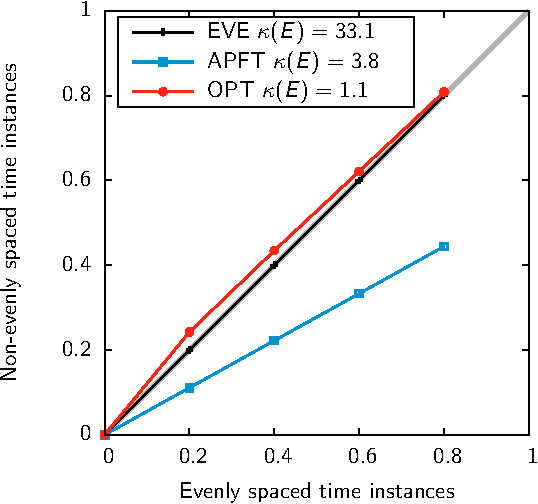
\includegraphics[width=.45\textwidth]{timelevels_distribution_f1.pdf}}
  \subfigure[relative to period $1/f_2$]{
      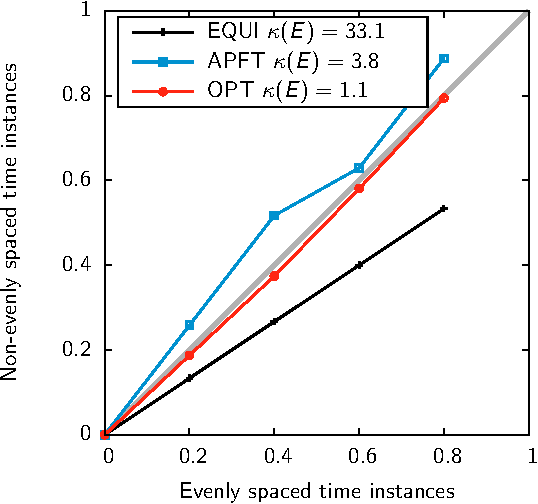
\includegraphics[width=.45\textwidth]{timelevels_distribution_f2.pdf}}
  \caption{Distribution of the time instances on each frequency periods.}
  \label{fig:distribution_tlv}
\end{figure}


% \section*{Summary}

% We have seen that the condition number of the
% discrete Fourier transform matrix $E$ can be large
% when using the multi-frequential framework. The present work,
% namely contra-rotating open rotor aeroelasticity, is
% by essence multi-frequential. It has been shown that in this context,
% the condition number has to be minimize for the harmonic balance
% computations to converge and the results to be reliable. 
% To ensure that, non-uniform time instances
% are used together with the OPT algorithm that provides an
% optimal condition number for any input frequencies.
